\section{An assignment model of elective surgical capacity}
\label{sec:model}

The empirical sections establish three facts that determine the structure of any
model of this system. Capacity is consumed in bed-days rather than cases, and
procedures differ systematically in how many bed-days they consume. Facilities
differ in how tightly that capacity binds, with municipal-administered units
operating near a third of total bed occupancy and state-administered units near
four fifths. And elective surgery is regionally organised: over 2019 to 2025, 42.7 per cent of elective admissions occur outside the patient's municipality of residence, and
state-administered facilities draw 70.3 per cent of their elective patients from
outside their host municipality against 30.4 per cent at municipal-administered
facilities.

We therefore formulate the allocation of elective surgery in Goi\'as as a
capacitated assignment problem with a travel-penalised access objective, and use
it to ask a counterfactual question: given the observed facility set, the constructed bed-day budget and historical peak-volume caps, what allocation of elective cases would have
delivered the same volume at least travel cost, and how far was the observed
allocation from it?

At the reported optimum, aggregate utilisation of the constructed net surgical
bed-day budget is 0.132 in 2019, 0.178 in 2023 and 0.215 in 2025, and one, three
and six facilities use more than 95 per cent of it, while the peak-volume cap is
reached far more often. Section~\ref{sec:capbind} reports this at the reported
optimum, and Section~\ref{sec:capnull} tests how much of it survives across
optima of equal cost and against counting noise; less survives than the reported
optimum suggests. Section~\ref{sec:decomp} describes how the attainable frontier moved: most of the improvement between
2019 and 2023 comes with the arrival of facility-procedure pairs absent in 2019 and the caps they carry,
though the split between options and capacity depends on the order of steps. Because the set of pairs itself changes, the fixed-machine-set restriction stated in
Section~\ref{sec:fixed} is a substantive question rather than a caveat.

\subsection{Sets and parameters}
\label{sec:sets}

Let $I$ index municipalities of residence, $J$ index facilities, and $P$ index
procedure subgroups at the four-digit SIGTAP level. Residents of municipalities
outside Goi\'as account for approximately 0.7 per cent of elective admissions and
are dropped, leaving $|I| = 246$. In 2019 and 2023, $|J| = 131$ facilities have
positive elective volume and non-zero net bed-day capacity; in 2025 there are
145. In every year $|P| = 16$.

\paragraph{Scope of the observed baseline.} The observed mean travel cost the
optimum is compared against is computed on admissions at facilities in $J$:
74{,}832 of the 79{,}247 in-state elective admissions of 2023, or 94.4 per cent.
The 5.6 per cent excluded had a higher mean cost index than the records retained, a mean of
1.003 index units against 0.846, so scoring the same optimum against the
all-records observed mean raises the estimated gap to 31.3 per cent rather than
the 30.6 per cent reported. The reported figure is the conservative one.

Demand $d_{ip}$ is the count of elective admissions of procedure type $p$ by
residents of municipality $i$ in the period. We treat observed admissions as a
lower bound on demand, since SIH records completed admissions and is silent on
patients who never reached surgery; Section~\ref{sec:limits} states what this
does and does not permit us to claim.

Throughout, $d_{ip}$, $B_j$ and $\kappa$ are monthly quantities (annual totals divided by twelve). Capacity $B_j$ is facility $j$'s surgical bed-day endowment: SUS surgical beds
from the CNES bed file multiplied by 30 days per month (calendar days per month, 30.4 on average, move the 2023 gap by +0.5 points), net of the bed-days
consumed by urgent surgical admissions at that facility. Netting all
non-elective bed-days, including clinical, obstetric and intensive care, against
surgical beds alone drives a third of facilities to zero capacity and is not the
correct pairing; numerator and denominator must both be surgical. Bed-day
consumption $\lambda_{jp}$ is the mean length of stay of procedure type $p$ at
facility $j$, estimated on observed admissions and shrunk toward the
procedure-level mean with weight $K=30$ where facility-procedure cell counts are
small.

Travel cost $c_{ij}$ is ordinal rather than metric, taking value $0$ if facility
$j$ lies in municipality $i$, $1$ if it lies in $i$'s IBGE immediate region,
$2$ if in $i$'s intermediate region, and $3$ otherwise. This uses IBGE immediate and intermediate geographic regions, which resemble but are not the CIB health regions (regi\~oes de sa\'ude) on which SUS referral agreements are written, and avoids
imputing road distances that the administrative data does not contain.

\paragraph{Metric robustness.} Replacing the ordinal cost with great-circle
distance between municipal seats raises the estimated gap rather than lowering
it, to 36.6 per cent in 2019, 39.7 in 2023 and 31.6 in 2025, against 28.8, 30.6
and 29.1 on the ordinal. The two constructs also largely agree on which
allocations are good. The ordinal-optimal 2019 solution carries 38.8 km per case
against a metric optimum of 31.5 and an observed 49.6; the metric-optimal
solution carries 0.634 index units against an ordinal optimum of 0.595. We
report the
ordinal figure throughout because it follows the IBGE regional hierarchy, which
resembles the health regions on which SUS referral is organised (official health
regions are a robustness row in Table~\ref{tab:measure}), and because it is the more conservative of the two.
Great-circle distance is itself a proxy: it ignores the road network, which in
interior Goi\'as can make actual travel substantially longer than the straight
line.

\subsection{Decision variables and formulation}
\label{sec:formulation}

Let $x_{ijp} \geq 0$ be the number of elective cases of type $p$ from
municipality $i$ performed at facility $j$, and let $u_{ip} \geq 0$ be unmet
demand. The program is

\begin{align}
\min_{x, u} \quad & \sum_{i,j,p} c_{ij}\, x_{ijp} \;+\; \pi \sum_{i,p} u_{ip} \label{eq:obj}\\
\text{s.t.} \quad & \sum_{j} x_{ijp} + u_{ip} = d_{ip} && \forall i, p \label{eq:demand}\\
& \sum_{i,p} \lambda_{jp}\, x_{ijp} \leq B_j && \forall j \label{eq:capacity}\\
& \sum_{i} x_{ijp} \leq m\,\kappa_{jp}, \quad \sum_{i,p} x_{ijp} \leq m\,\kappa_{j} && \forall j, p \label{eq:cap}\\
& x_{ijp} = 0 && \forall (j,p) \notin S \label{eq:scope}\\
& x_{ijp}, u_{ip} \geq 0. \nonumber
\end{align}

Constraint~\eqref{eq:demand} conserves demand. Constraint~\eqref{eq:capacity} is
the bed-day budget: this is where the length-of-stay result enters, since a
facility that treats a given case mix with longer stays exhausts its budget at
fewer cases. Constraint~\eqref{eq:cap} is the historical peak-volume cap,
described below. Constraint~\eqref{eq:scope} restricts each facility to the
procedure types it has been observed to perform, with the scope set $S$ taken
from observed activity in the estimation window rather than assumed. The scope
set closes 73 per cent of the assignment space, counted over the full
$|I| \times |J| \times |P|$ grid of 515{,}616 triples; the number of facilities
performing a given subgroup ranges from 5 to 97. The program is built only over
demand cells that are non-empty, so the variable count reported in
Section~\ref{sec:modelresults} is smaller again.

\paragraph{The peak-volume cap.} $\kappa_{jp}$ and $\kappa_{j}$ are facility $j$'s
peak 3-month average volume in the estimation year, for procedure $p$ and in total. This is
a historical high-water mark, a lower bound on what the unit has delivered and not a measured
ceiling on what it can deliver (Section~\ref{sec:capnull}); we call it a cap because the program
imposes it as one. The natural construction is the largest monthly caseload observed in the estimation year.
Bounding facility throughput by observed case volume in this way is in the spirit of
\citet{vogel2022}, who constrain each hospital to a multiple of its base-year
volume when simulating minimum volume regulation in the German hospital sector;
our multiplier ladder in Table~\ref{tab:modelrobust} plays the same role as
their $v_{\max}$. Section~\ref{sec:data} documents batch reporting in SIH, and a facility that
bills two months of work in one produces a maximum that overstates what it can
do. In 2023, 37 of the 136 facilities with positive elective volume report
interleaved zero months within their span, carrying 12.4 per cent of elective
volume, and their ratio of single-month maximum to three-month rolling maximum
is 1.53 against 1.21 for the rest. The count is 136 rather than the $|J| = 131$
of Section~\ref{sec:sets} because five facilities with elective volume in 2023
have no net surgical bed capacity once urgent consumption is deducted, and are
not carried into the program. We therefore define $\kappa$ as the largest
three-month rolling mean of monthly volume, applied uniformly to every facility
rather than only to those classified as batch reporters, so that the rule does
not condition on a classification we constructed. This tightens total cap
capacity by 20 per cent relative to the single-month maximum and lowers the
reported gaps; the single-month rule is reported as a robustness row.

Pairs whose rolling mean falls below half a case per month are given a floor of
$0.5$, so that a pair observed to exist is not assigned a cap of effectively
zero. The floor is a construct rather than a measurement, and pairs subject to it
are excluded from every pair-level count reported below. They are not a small
group: of the pairs carrying positive flow at the optimum, 116 of 532 are floored
in 2019, 111 of 601 in 2023 and 100 of 663 in 2025, between a sixth and a fifth
of the option set in use. Their share of served volume is small, falling from
1.3 per cent in 2019 to 0.7 and then 0.5, because a floored pair is by
construction one that carries almost no volume. Their shadow prices are not
small, however, and Section~\ref{sec:capbind} reports the consequence: because
the floor is a construct rather than a measurement, a floored pair at its cap
should not be read as a facility at the limit of what it can do.

Every pair-level share reported below therefore has as its denominator the pairs
that carry positive flow at the optimum and are not floored: 416 of 563 scope
pairs in 2019, 490 of 637 in 2023 and 563 of 704 in 2025. The gap between scope
and use is the pairs the optimum declines to employ at all, 31, 36 and 41
respectively. A pair is counted as binding when it carries more than 95 per cent
of its cap.

\paragraph{What the peak-volume cap restricts.} Equation~\eqref{eq:cap} has two
rows, and they do different work. Dropping the pair row and retaining only the
facility total isolates them. With no peak-volume constraint at all the gap is
50.4 per cent in 2019, 56.1 in 2023 and 56.4 in 2025. Imposing only the facility
total takes it to 35.5, 39.4 and 40.1. Imposing the pair row as well takes it to
28.8, 30.6 and 29.1. The first step, worth 14.9, 16.7 and 16.3 points, is the effect of the facility-total cap. The
second, worth 6.7, 8.8 and 11.0 points, is the effect of the pair-level cap. The facility-total step is the larger throughout, but the pair-level step grows across the panel, from 31 to 35 to 40
per cent of the combined restriction. Both rows therefore restrict the benchmark, and the pair row's share grows across the panel.

This matters for how a shadow price on $\kappa_{jp}$ should be read. Where the
facility total also binds, relaxing one pair's cap moves volume within the
facility rather than adding to it, so the pair's dual is not the value of new
capability at that pair alone. That is the majority case: of the pairs carrying a
positive dual, 62 per cent in 2019, 55 in 2023 and 79 in 2025 sit at a facility
whose total cap is also binding. Section~\ref{sec:placement} conditions on this
rather than ranking on the raw dual.

The penalty $\pi$ prices unmet demand against travel. It is the only parameter
in the program with no empirical referent: the shrinkage weight $K = 30$, the
$0.5$ floor and the three-month rolling window are also chosen rather than
estimated, but each is a construction applied to observed quantities, whereas
$\pi$ is a price the data does not contain. Where the program serves all demand, $\pi$ does not enter the
solution at all. Where capacity binds, we report results across $\pi \in
\{4, 6, 10\}$ and show in Section~\ref{sec:decomp} that the ordering of
configurations is invariant over that range.

\paragraph{Comparing configurations that leave demand unmet.} Mean travel cost
over served cases is not comparable across configurations with different unmet
volume. When capacity binds, the program chooses which demand to leave unserved,
and it drops the cells whose nearest permitted facility is farthest; the served
pool is then a closer, selected subset and its mean travel falls mechanically.
Tightening capacity can therefore appear to improve routing. We report instead
an adjusted cost that charges unmet demand at $\pi$ and divides by total rather
than served demand,
\[
\bar{c}^{\,\text{adj}} \;=\; \frac{\sum_{i,j,p} c_{ij} x_{ijp} \;+\; \pi \sum_{i,p} u_{ip}}{\sum_{i,p} d_{ip}},
\]
which is the objective value per unit of demand and is defined on the same
denominator in every configuration. Where unmet demand is zero the two measures
coincide.

\subsection{What the model does and does not treat as fixed}
\label{sec:fixed}

The machine set is fixed within a period, and this is the model's central
restriction rather than an incidental one. Appendix~\ref{sec:appb2} establishes that the set of facility-procedure pairs changes from year to year: 284 pairs
present in 2023 are absent in 2019 and 192 go the other way, and most of the 284
had earlier activity in the record. A model that cannot open or close pairs therefore
cannot represent the change in the set of pairs through which this system expanded. We
solve the model period by period on the capacity that existed in that period,
and read the within-period gap as the distance between the observed allocation and the benchmark for that period's pairs and caps.
Section~\ref{sec:decomp} then relaxes the restriction across periods to
describe how the frontier moved.

Urgent demand is not modelled explicitly. It enters through $B_j$, which is net
of the bed-days consumed by urgent surgical admissions at each facility in the
period. This is why urgent use matters for the solution rather than merely describing it: a facility with heavy urgent surgical use contributes a smaller bed-day budget than its bed count suggests.

\subsection{Results}
\label{sec:modelresults}

We solve the program on three years: calendar 2019, the last full pre-pandemic
year and the baseline the empirical sections establish as the appropriate
counterfactual; calendar 2023; and calendar 2025, the most recent complete year
in the data. The 2019 instance has 246 municipalities of residence, 131
facilities and 16 procedure subgroups, giving 99{,}025 assignment variables over
2{,}294 demand cells; the 2025 instance is the largest, with 145 facilities and
704 facility-procedure pairs in scope. All three solve to optimality in
seconds.

The observed 2019 allocation carries a mean travel cost of 0.835
index units per elective case. The unconstrained optimum delivers identical
volume, with no unmet demand, at 0.414: a reduction of 50.4 per cent. This
figure should not be the headline, because with bed-days slack almost everywhere
the program is free to route demand to any facility within its observed scope,
including facilities that performed the procedure only a handful of times.
Table~\ref{tab:modelrobust} therefore reports the ladder of peak-volume caps.

\begin{table}[t]
\centering
\caption{Optimal mean travel cost under increasingly tight caps on facility
throughput. The cap restricts each facility to a multiple of its largest
three-month rolling mean monthly elective caseload in the estimation year. All
specifications serve the full observed volume with zero unmet demand, so the
adjusted and served-only costs coincide throughout.}
\label{tab:modelrobust}
\begin{tabular}{lrrrrrr}
\toprule
& \multicolumn{2}{c}{2019} & \multicolumn{2}{c}{2023} & \multicolumn{2}{c}{2025} \\
\cmidrule(lr){2-3}\cmidrule(lr){4-5}\cmidrule(lr){6-7}
Specification & Cost & Reduction & Cost & Reduction & Cost & Reduction \\
\midrule
Observed allocation & 0.835 & --- & 0.846 & --- & 0.906 & --- \\
Unconstrained optimum & 0.414 & 50.4\% & 0.372 & 56.1\% & 0.395 & 56.4\% \\
Cap at 2$\times$ historical peak & 0.513 & 38.6\% & 0.474 & 43.9\% & 0.518 & 42.8\% \\
Cap at 1.5$\times$ historical peak & 0.542 & 35.1\% & 0.507 & 40.1\% & 0.551 & 39.2\% \\
Cap at 1$\times$ historical peak & 0.595 & 28.8\% & 0.587 & 30.6\% & 0.642 & 29.1\% \\
\midrule
\multicolumn{7}{l}{\emph{Robustness: single-month maximum in place of three-month rolling mean}} \\
Cap at 1$\times$ historical peak & 0.537 & 35.7\% & 0.509 & 39.9\% & 0.559 & 38.2\% \\
\bottomrule
\end{tabular}
\end{table}

The result to take is the 1$\times$ row. Constraining every facility to do no more per month than its highest recorded three-month average, the
same volume of elective surgery could have been delivered in 2019 at 0.595
index units per case against an observed 0.835, a reduction of 28.8 per cent. The observed allocation respects the caps by construction but exceeds the bed-day budget at 1, 2 and 4 facilities, so it is not strictly a feasible point of the program and the sign of the gap is not guaranteed by construction; the gap measures distance under the program's rules, and we offer no threshold for what size would indicate a problem. This specification needs no outside estimate of capacity: each facility is held to its own
peak 3-month average volume. It does assume that this historical peak is a feasible level for the unit. Just over half of the
unconstrained gain survives the binding cap: 0.240 of 0.421 index units in
2019, and 54.6 and 51.7 per cent of it in 2023 and 2025.

The later columns are the more striking ones. The observed mean index did not fall
across the panel; it rose, from 0.835 in 2019 to 0.846 in 2023 and 0.906 in
2025, while elective volume more than doubled. The optimum under the
cap moves little against that: 0.595, 0.587, 0.642. The point estimates of the
gap are close, 28.8, 30.6 and 29.1 per cent, and the differences between years
are not distinguishable from zero (Section~\ref{sec:uncertainty}); the intervals are too
wide to establish that the gap was constant. Municipal rankings of excess ordinal cost
are correlated across years, at 0.68 to 0.74 (Section~\ref{sec:flows}). We do not
attribute the absence of a detectable change to any reform.

Two qualifications belong with the number. Travel cost here is an ordinal index (0 to 3), not kilometres and not a count of region
crossings, so a ratio of its means has no distance interpretation; the gap is a statement about
the index, and its level depends on the coding (Section~\ref{sec:capnull}). And the model routes on procedure
subgroup and observed scope alone; it does not observe surgeon subspecialty,
equipment, or the case-volume thresholds that clinical governance may impose
within a subgroup. Some part of the observed cost index is therefore a constraint the
data does not record. The peak-volume cap absorbs the facility-level version of
this concern but not the procedure-specific version.

\subsection{How the attainable frontier moved between 2019 and 2023}
\label{sec:decomp}

The two years differ in three respects that the ladder above cannot separate:
demand is larger in 2023, capacity is larger, and the set of facility-procedure
pairs is larger, 637 against 563. We separate them by solving four
configurations, each combining a demand year with an option set and a capacity
vintage. Table~\ref{tab:decomp} reports them.

\begin{table}[t]
\centering
\caption{Decomposition of the 2019--2023 frontier. Adjusted cost charges unmet
demand at $\pi$ and divides by total demand; see Section~\ref{sec:formulation}.
Configurations A and D serve all demand, so their adjusted and served-only costs
coincide.}
\label{tab:decomp}
\begin{tabular}{llrrrr}
\toprule
& Configuration & Options & Served-only travel & Adjusted cost & Unmet \\
\midrule
A & 2019 demand, 2019 options, 2019 capacity & 563 & 0.595 & 0.595 & 0.0\% \\
B & 2023 demand, 2019 options, 2019 capacity & 563 & 0.725 & 1.823 & 20.8\% \\
C & 2023 demand, 2019 options, 2023 capacity & 554 & 0.775 & 1.375 & 11.5\% \\
D & 2023 demand, 2023 options, 2023 capacity & 637 & 0.587 & 0.587 & 0.0\% \\
\bottomrule
\end{tabular}
\end{table}

Configuration C carries 554 options rather than A and B's 563 because the option
set is intersected with the capacity vintage it is solved against: five
facilities with 2019 elective volume have no net surgical bed capacity in 2023,
removing fourteen pairs, while one facility with 2019 volume and no 2019 net
capacity acquires some by 2023, adding five.

Configurations C and D differ only in which facility-procedure pairs are permitted: 554 against 637, on identical
demand and identical capacity. With the 2019 pairs 11.5 per cent of the 2023 demand is unserved and travel over the cases served is 0.775; with the 2023 pairs
all demand is served at 0.587. We do not attribute the change between options and capacity. The pairs absent in 2019 and the caps they carry arrive together,
and any split depends on the order of steps and on the penalty $\pi$ that prices unmet demand; the table reports served-only travel and the unmet share separately for that reason.

The option set did not simply accumulate. Between 2019 and 2023 the state gained
284 facility-procedure pairs and lost 192, a gross churn of 476 against a net
change of 92, both counted at the four-digit level at which the model routes.
This strengthens rather than weakens the comparison: configuration C is solved on
the 2019 option set including the pairs that later disappeared, so the
improvement from C to D is net of the exits, not gross of them.

Configuration B adds the 2019 capacity vintage to the 2019 option set and leaves
a fifth of 2023 demand unserved. The 2019 option set was generous relative to
2019 volume, in the sense that configuration A serves all demand with just over
half of the unconstrained gain still available, and binding relative to 2023
volume.

The ordering A $\approx$ D $<$ C $<$ B holds at $\pi = 4$, $6$ and $10$.
Configurations A and D serve all demand, so $\pi$ does not enter them.
Configuration B's allocation is identical at all three values and only the charge
on a fixed quantity of unmet demand changes. Only configuration C reallocates,
with unmet demand moving from 11.8 to 11.5 to 11.4 per cent as $\pi$ rises
through 4, 6 and 10, and configuration B's from 21.2 to 20.8. The decomposition
is therefore not an artefact of the penalty.

\subsection{Beds and the peak-volume cap at the reported optimum}
\label{sec:capbind}

Table~\ref{tab:decomp} shows that with the 2023 pairs and caps all 2023 demand is assigned. The ratio of aggregate cap to demand did not rise.
Capability capacity, the sum over facilities of the rolling-mean cap, rose 64.9
per cent between 2019 and 2023 against a 70.7 per cent rise in demand.
Aggregate peak-volume cap exceeded demand by a factor of 1.368 in 2019, 1.321 in 2023
and 1.160 in 2025. Surgical bed-days rose 20 per cent between the first two
years. At the pair level, 233 of 416 facility-procedure pairs bind at the 2019
optimum, 249 of 490 in 2023 and 339 of 563 in 2025, carrying 54.5, 46.0 and 54.4
per cent of served volume. The option set expanded at approximately the rate
demand did through 2023 and more slowly thereafter, so the ratio of aggregate peak-volume cap to demand falls rather than rises: by 2025
the cap exceeds demand by 16 per cent against 37 per cent in 2019. Section~\ref{sec:capnull}
asks what the fall consists of.

Two utilisation measures appear below and they are not the same quantity.
\emph{Aggregate} bed utilisation is state-wide bed-days used over state-wide
bed-days available, and is the series reported in this subsection and in Section~\ref{sec:capnull}. \emph{Mean facility utilisation} is the
unweighted mean of facility-level ratios over a named subset of facilities, and
is always smaller here because the facilities holding the most spare capacity are
small.

The two constraints bind on almost disjoint sets of facilities. In 2023 three
facilities use more than 95 per cent of their bed-day budget, and those three operate at
0.58 of their peak-volume cap. At the reported optimum 77 facilities are at their cap, with mean
facility utilisation 0.116, and hold 26{,}269 unused surgical bed-days per month
between them, against 10{,}902 bed-days consumed per month by all 131 facilities
in the solution. The two figures have different denominators and their ratio is
not a utilisation rate; aggregate bed utilisation in the same solution is 0.178.
In 2019 one facility reaches its bed-day budget, at 0.41 of its peak-volume cap,
while 79 reach their peak-volume cap at mean facility utilisation 0.115 and hold
23{,}821 spare bed-days. In 2025 six facilities are bed-bound at 0.63 of their
peak-volume cap, while 105 of 145 are at their peak-volume cap at mean facility
utilisation 0.149 and hold 31{,}309 spare bed-days.

At the reported optimum no facility is both bed-bound and at its peak-volume cap in 2019 and 2023, and
144 of 145 facilities are not both in 2025. The exception is CNES 2382474 in S\~ao Lu\'is de Montes Belos, which in the
2025 solution reaches bed utilisation 1.000 and cap use 0.985 simultaneously.
The 2025 overlap is not a trend: in the 2019 optimal face a facility can already be both bed-bound and at cap
(Section~\ref{sec:capnull}), so an overlap appearing in 2025 at this vertex does not mark a leading edge. The ratio of aggregate peak-volume
cap to demand falls from 1.368 to 1.160 and state-wide bed utilisation moves from 0.132 to 0.178 to 0.215, and the facilities at their cap
are, at the reported optimum, mostly ones with bed-days to spare. The share of pairs that bind is not monotone, at 56.0, 50.8 and 60.2 per cent.
Beds, counted at full occupancy, are not scarce at any of the three dates in this program; operating-room sessions, surgeons and
anaesthetists are not modelled.

Read with Section~\ref{sec:results}, this describes the expansion without identifying its cause. Bed utilisation rose only from 0.13 to 0.21
while elective volume more than doubled, and routing showed no detectable improvement. What changed in the record is the set of active facility-procedure pairs,
most of them pairs with earlier activity in 2020 to 2022 (Appendix~\ref{sec:appb2}).
Whether the right response is to place capability or to change how existing capability is used is a policy question this model does not answer.

\subsection{What the peak-volume cap is, and what survives}
\label{sec:capnull}

The cap $\kappa$ is a peak: the largest 3-month average of a unit's own monthly volume in the estimation year. A maximum over
windows exceeds the mean mechanically, so several statements about it need a test against what noise alone would produce. This
subsection reports those tests. A record of when each rule was written relative to its results is in the repository (\texttt{dist/sprint/PREREG\_CHRONOLOGY.md}); only some were committed before their results existed.

\paragraph{The at-cap count is not identified.} The program's optimum is a face, not a point: many allocations have the same
cost. We searched that face (cost within $10^{-9}$ of optimal; a margin of $10^{-4}$ of the cap for a facility to count as at cap; 200 seconds per
search; every count quoted in a row comes from one solution, and no row constraint was violated by more than $10^{-14}$ in relative terms). The number of facilities using more than 95 per cent of their
peak-volume cap has a proved minimum of 34 of 131 in 2019, 44 of 131 in 2023 and 64 of 145 in 2025. The largest value found is 101, 107 and 115, with upper bounds of
113, 108 and 131 that the solver did not close. At 90 per cent the proved minimums are 39, 52 and 69, and at 99 per cent 31, 43 and 53. At the reported optimum (the stored solution) the counts are 79, 77 and 105; a fresh solve of the same program lands on another vertex with 72, 75 and 103, which is the non-uniqueness at work. Bed-bound facilities (more than 95 per cent of the
bed-day budget) range from 0 to 2 in 2019 (proved), from 2 to at least 4 (upper bound 5) in 2023 and from 4 to at least 7 (upper bound 9) in 2025, against 1, 3 and 6 at the reported optimum (1, 3 and 5 at the fresh solve). Statements about how many facilities ``are at their cap'' are therefore statements about one optimum among many. The unused surgical
bed-days at facilities at cap are at least about 9{,}700 (2019) and 12{,}100 (2023) at some optimum; we did not establish their upper range at these settings, so the 26{,}269 bed-days
quoted earlier for 2023 is the value at the stored solution only.

\paragraph{Disjointness.} At the reported optimum the two constraints bind on disjoint sets of facilities in 2019 and 2023 and overlap at one facility in 2025. Across the optimal
face, an overlap of one facility is attainable in 2019 (proved) and of two in 2025 (found; the solver could not rule out more, with an upper bound of five). In 2023 no overlap
was found, but the search did not prove that none exists (upper bound two within the time limit). Disjointness is therefore a statement about the reported optimum and not about
the face. How informative it is against chance depends on the vertex: with $K$ bed-bound and $n$ at-cap facilities among $N$, the probability under random assignment of an overlap as small as the one
observed ranges across the extreme vertices from 0.23 to 0.80 in 2019, 0.03 to 0.19 in 2023 and 0.001 to 0.17 in 2025 (0.40, 0.07 and 0.006 at the reported optimum). In 2019 the minimum number of
bed-bound facilities across the face is zero, so the claim can be vacuous there.

\paragraph{The cap test.} If caps bind, units at their cap in year $t$ should be exceeded less often in year $t+1$ than a
stationary system would exceed them. Among facilities at cap, 51.3 per cent (2023 to 2024) and 52.4 per cent (2024 to 2025) have a
larger peak the next year. Rebuilding the peak, re-solving the program and redefining ``at cap'' on 200 simulated stationary years,
that rate is 45.9 per cent (95 per cent range 35.5 to 53.8; $p = 0.13$) and 44.2 per cent (36.4 to 53.6; $p = 0.05$) when each unit's
months are Poisson, and 47.9 per cent (36.3 to 58.1; $p = 0.24$) and 47.7 per cent (37.5 to 56.9; $p = 0.18$) when each facility's
months are resampled from its own observed months, which keeps its overdispersion. The observed rates are inside the null range. This is a
low-power non-rejection: it is not evidence that the cap binds and not evidence that it does not. The contrast between the at-cap and not-at-cap rates
(observed $+0.17$ and $+0.21$) is also inside the null range (Poisson $+0.04$ with range $-0.28$ to $+0.34$, $p = 0.21$, and $-0.14$ with $-0.60$ to $+0.40$, $p = 0.07$; resampling $+0.07$
with $-0.11$ to $+0.24$, $p = 0.13$, and $+0.07$ with $-0.11$ to $+0.25$, $p = 0.06$). Restricting to the 43 facilities that are at cap in every optimum of equal cost in 2023 (a fixed set, so the null does not simulate the
selection), 55.8 per cent exceed their cap in 2024 against a null of 43.4 per cent (27.9 to 58.1; $p = 0.07$). The size of the exceedance is larger than the resampling null produces
(a median of 71 and 54 per cent of the cap, against 19 and 21 per cent), but this test does not separate growth in demand from a cap that was never binding, and we
claim neither. Where the CNES count of registered surgeons rose, at-cap facilities exceeded their cap in 79 and 63 per cent of cases against null rates of about 48 and 50 per cent; we treat this as
exploratory and unidentified: it is a registration count, it does not control for facility growth, and the urgent-volume placebo shows no such excess.

\paragraph{What the ratio of cap to demand contains.} The aggregate ratio of caps to demand (1.368, 1.321, 1.160) is not slack in
the sense of unused capacity. The sum of caps over the sum of mean volume at the same facilities is 1.37, 1.40 and 1.27, and the expected maximum 3-month mean of twelve Poisson months at those means would alone give a
ratio of about 1.09 (the one floor we use), so about a quarter of the excess over one exists by construction. We tested whether the fall in the ratio reflects flatter monthly series, with a rule stated for the
2019-to-2025 comparison: the volume-weighted peak-to-mean ratio net of that floor, over the 96 facilities present in both years, changes by $-0.07$ (95 per cent facility-bootstrap interval $[-0.15, +0.01]$). The interval includes
zero, so the explanation ``flatter months'' is not supported. The 2019-to-2023 fall coincides with falling coverage (the facilities in the model account for 100, 94 and 91 per cent of demand). A 2023-to-2025 contrast, chosen after seeing the
full-period result, gives $-0.12$ ($[-0.22, -0.05]$) and is exploratory. We do not describe the fall as a tightening of capacity.

\paragraph{Measurement choices.} Table~\ref{tab:measure} reports the gap when the inputs are rebuilt differently. The gap is robust
to defining months by discharge date and, in 2019 and 2023, to the estimation window. It is not robust to the cost coding (an
ordinal index counting municipality as a step: 29 to 31 per cent; boundary crossings only: 37 to 41 per cent), to the bed-day
definition (netting all admissions against all inpatient beds admits more facilities and gives 29, 37 and 40 per cent) or, in 2025, to
the window (25 per cent for July to June). Bed utilisation stays low under every definition (0.06 to 0.22, each definition solved afresh) and at most one facility is bed-bound when all admissions are netted against all inpatient beds, but the bed row is not inert: dropping it raises the gap by 0.0, 3.5 and 2.4 points (2019, 2023, 2025) because 1, 3 and 5
facilities would then exceed their bed-day budget, while replacing the shrunk stay lengths by facility-procedure means leaves the gap unchanged (0.0, 0.0 and $-0.1$ points). Beds are slack in aggregate and bind at a few facilities.
Observed elective bed-days exceed the budget at 1, 2 and 4 facilities. Batch
reporting is not the main source of month-to-month variation: defining months by discharge date lowers the number of facilities with
interleaved zero months only from 45 to 38 and from 36 to 31, so the rolling three-month mean is a smoother, not a correction for a
processing artifact. Zone size matters in the same direction. Aggregating origins to the IBGE immediate region, with cost 0 for a facility in the same region, is the same program as the boundary-crossing recoding (cost then depends only on the origin's region) and gives 37.1, 39.9 and 41.0 per cent; aggregating to the IBGE intermediate region to 38.1,
47.1 and 51.0, because a coarser zone hides which patients already travel within their zone; the gap is zone-dependent by more than five
points at every zone size. The gap computed against all in-state records, rather than records at model facilities, is 28.8, 31.3 and 29.0
per cent, within 0.7 points of the headline.

\paragraph{The gap depends on the cap.} The cap is built from the same months it constrains and is a peak, so each pair is given
headroom of peak over mean. Replacing the peak with the unit's annual mean volume (the fixed-marginal benchmark of the
excess-commuting literature) leaves almost nothing to reallocate in 2019, a gap of 6.2 per cent with 0.3 per cent of demand unserved; in 2023 the gap is
22.7 per cent with 7.3 per cent unserved and in 2025 29.6 per cent with 9.8 per cent unserved, so those are not like-for-like. Deflating the peak by
the expected excess of the maximum of twelve Poisson months over their mean gives 22.7, 24.0 and 24.8 per cent, 6.0, 6.5 and 4.3 points below the
headline. The headline gap is therefore partly headroom that a peak always has over a mean, and is reported with this bracket.
Bed utilisation is not an artifact of the cap: it is 0.12, 0.178 and 0.198 at the 2$\times$ cap and 0.129, 0.188 and 0.199 with no cap (2019, 2023,
2025), against 0.132, 0.178 and 0.215 at 1$\times$. Across the optimal face it ranges from 0.122 to 0.166, 0.165 to 0.217 and 0.206 to 0.238.


\begin{table}[t]
\centering
\caption{The gap (per cent) under alternative constructions of the inputs; reported-optimum values. The July-to-June window needs the
preceding year, so 2019 is not available; discharge-month results for 2025 are omitted because the files that would complete December
2025 do not exist.}
\label{tab:measure}
\small
\begin{tabular}{p{0.60\textwidth}rrr}
\toprule
Construction & 2019 & 2023 & 2025 \\
\midrule
Paper (month of processing, calendar year, ordinal cost) & 28.8 & 30.6 & 29.1 \\
Month of discharge (DT\_SAIDA) & 29.1 & 29.0 & --- \\
July-to-June window & --- & 30.5 & 25.2 \\
Actual days per month in the bed budget & 28.8 & 31.1 & --- \\
All admissions netted against all inpatient beds & 28.9 & 36.9 & 40.3 \\
Boundary-crossing cost (0/0/1/2); same as origin zone = IBGE immediate region & 37.1 & 39.9 & 41.0 \\
Origin zone = IBGE intermediate region (cost 0/1) & 38.1 & 47.1 & 51.0 \\
Baseline over all in-state records & 28.8 & 31.3 & 29.0 \\
Residents of the 29 RIDE-DF Entorno municipalities excluded & 29.6 & 32.3 & 28.5 \\
Official health regions (SES-GO, 18) replace IBGE regions in the cost & 30.7 & 35.1 & 30.7 \\
Origin zone = health region (cost 0/1/2) & 39.0 & 47.5 & 43.7 \\
Origin zone = health macro-region (cost 0/1) & 44.3 & 51.3 & 54.6 \\
\bottomrule
\end{tabular}
\end{table}

\subsection{Where the gap falls}
\label{sec:flows}

The aggregate gap conceals an allocation. The 2023 optimum assigns 2{,}908
origin-facility-procedure flows, and ranking municipalities of residence by excess ordinal cost, the difference between observed and optimal mean cost weighted by
served volume, locates the gap geographically. Total excess is 1{,}668 cost
units per month across 246 municipalities. The fifteen largest origins carry 44.6
per cent of net total excess (44.3 per cent of the sum of the positive entries, the denominator
used when negative entries are set aside).

Two properties of this measure should be stated before it is read. Excess weights
each municipality by the volume the optimum assigns it, while the aggregate
observed mean of Section~\ref{sec:modelresults} weights by observed admissions at
facilities in $J$; the two coincide in 2019 and diverge by 2025, where the
observed mean is 0.919 under the first weighting and 0.906 under the second, so
total excess is not the product of the headline gap and total volume. And excess
is not a partition: a municipality whose observed allocation is more local than
the peak-volume caps permit the optimum to be takes a negative value, so the
positive entries sum to more than the aggregate gap. The negative entries are
small in the first two years and not in the third, at 0.0 per cent of the
positive total in 2019, 0.6 in 2023 and 5.1 in 2025. The 2025 figure is almost
entirely one municipality, which alone accounts for $-81.9$ of the $-118.1$ total across
seven municipalities. The artifact is therefore contained rather than systematic,
but it is concentrated in exactly the municipality the ranking below singles
out, and that ranking should be read with this in mind. The 2019 and 2025 optima
assign 2{,}600 and 3{,}125 flows, with total excess of 929 and 2{,}211 units and
fifteen-largest shares of 42.5 and 49.9 per cent of net excess (42.5 and 47.3 per cent of the sum of positive entries). Total excess grows with volume
and concentrates as it grows, even though the gap expressed as a share of the observed cost index does not.

In the reported optimum these origins are assigned to lower-cost facilities than the ones recorded. Rio Verde, the largest
single contributor at 107.6 units, sends its residents to facilities with a mean
cost of 0.75 against 0.20 in the reported optimum, and the optimal assignment
routes almost all of that volume to two facilities in Rio Verde itself. An\'apolis
moves from 0.24 to 0.06 by treating its residents at a facility in An\'apolis.
Jata\'i moves from 1.21 to 0.30 the same way. Across the state, 67.2 per cent of
optimal flow is served in the patient's own municipality in 2023, against 68.7
per cent in 2019 and 63.1 per cent in 2025. In the reported optimum the model assigns these municipalities' residents to local facilities at lower cost; this does not establish that those facilities could absorb the caseload or that observed flows are misallocation.

Two origins behave differently. \'Aguas Lindas de Goi\'as and Valpara\'iso de Goi\'as
retain optimal costs of 1.68 and 1.55 in 2023, the highest among the largest
contributors. Both lie in the Entorno do Distrito Federal. Within SIH Goi\'as the binding
constraint for both is the absence of a local pair rather than its misuse, but this cannot be read as a finding
about the Entorno: residents of Goi\'as treated in Distrito Federal hospitals appear in the DF files, not in SIH
Goi\'as, and in 2023 that is 25 per cent of the elective surgical admissions of the residents of
\'Aguas Lindas, Valpara\'iso and Luzi\^ania combined (51 per cent in 2019, 31 per cent in 2025). Their demand here is
therefore incomplete, and so is any conclusion about openings in the Entorno.

\begin{figure}[t]
\centering
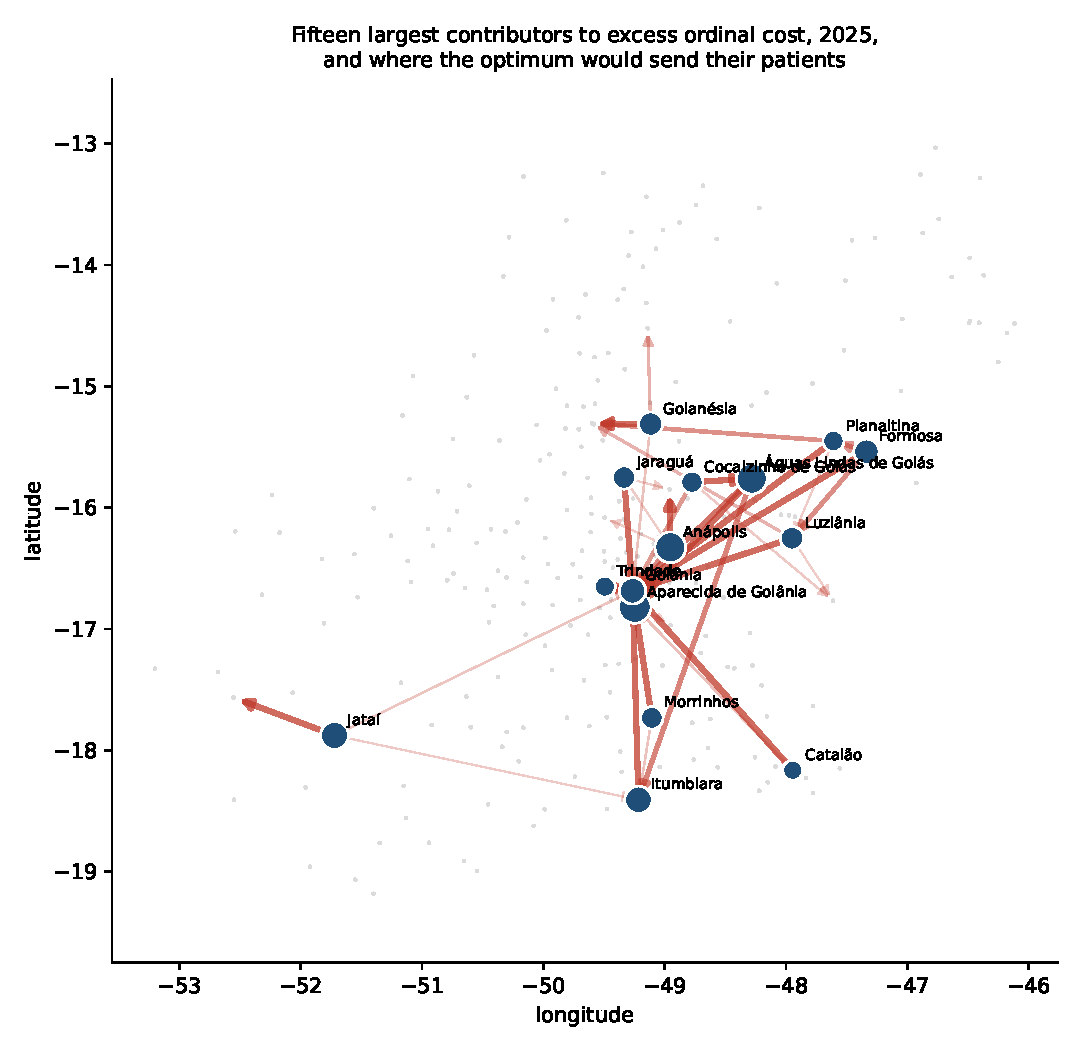
\includegraphics[width=0.82\textwidth]{fig4_worst_served_2025.pdf}
\caption{The fifteen municipalities contributing most to excess ordinal cost in 2025,
sized by that contribution, with arrows to the three municipalities the optimum
sends most of their volume to. Grey points are the remaining municipal seats.
Most arrows are short: the reassignment the model proposes is largely local.}
\label{fig:worst}
\end{figure}

The two diverge afterwards, in a way that illustrates the pattern at the scale
of a single municipality. Valpara\'iso has no facility with elective volume at
any of the three dates; its optimal cost falls from 2.42 to 1.55 and then holds
there, moving only because provision elsewhere moved nearer, and none of its
volume is served at home in any solution. \'Aguas Lindas acquires one facility
in SIH Goi\'as between 2019 and 2023, carrying two facility-procedure pairs, and six pairs by
2025; the optimum keeps none of its volume locally in 2019, 32 per cent in 2023
and 70 per cent in 2025, and its optimal cost falls from 2.54 to 1.68 to 0.91. The arrival of one facility carrying two facility-procedure pairs moves that municipality most of the way to the frontier in the model.

The ranking is positively correlated across the panel. The Spearman rank correlation of excess ordinal cost across the 246 municipalities is 0.737 between 2019 and 2023, 0.685
between 2023 and 2025, and 0.675 between the endpoints; ten, ten and eight of
the fifteen largest contributors carry over between the same pairs of years.
Aparecida de Goi\^ania is among the three largest at every date and An\'apolis
among the four, with the same structure throughout: observed cost well above an
optimum attainable within the patient's own municipality. The distance from the program's optimum recurs in these municipalities across the years examined; whether it reflects misallocation, patient choice, surgeon availability or regulation is not determined here. These municipal figures are computed at a single optimum of the program; a post hoc check in the repository (\texttt{dist/research2/RESULTS.md}, Addendum~3), which did not examine municipalities, finds that quantities below the state level (tested at the health-region level) are identified only at the exact optimum and not among allocations within 1 per cent of it, so the municipal ranks and shares describe the solution reported rather than every near-optimal allocation.

One large contributor does not persist, and the exception is instructive. Rio
Verde ranks first in both 2019 and 2023, at 69.8 and 107.6 units, and last of 246
in 2025 at $-81.9$. Its residents' observed mean cost fell from 0.75 to 0.40 while
their volume rose from 197 to 559 cases per month, and the peak-volume cap summed
over facilities in Rio Verde rose from 223 to 477 cases per month across the same
interval. The excess turns negative because the caps now bind there: the optimum can keep
only 70 per cent of Rio Verde's volume in the municipality, against 96 per cent
in 2019, while observed practice keeps more, so the optimum's mean cost of 0.54
sits above the observed 0.40. This is a property of the
cap rather than evidence of over-performance. A facility may exceed its
three-month rolling mean in an individual month, and where it does, the observed
allocation is locally cheaper than any allocation the model is permitted to
choose. The largest single
distance from the optimum of the first two years closed, in the direction of the
model's ranking, with capability arriving where the patients already were. We do
not claim the model caused this; the quantity it ranks is one that
moves.

\subsection{Uncertainty and the equity margin}
\label{sec:uncertainty}

Every figure above is a point estimate on a single realised panel. We resample
facility-months, re-estimate $\lambda_{jp}$ and the caps on the resampled panel,
and re-solve at the 1$\times$ cap. Two procedures run on the same scheme and
should not be confused: a marginal bootstrap of 300 draws per year, reported
first, and the paired bootstrap of 340 replicates reported below, in which one
weight vector is applied to all three years at once. The scheme is a multiplier
bootstrap: $\kappa$ is a maximum over rolling windows, so any resample that
zeroes facility-months deflates it mechanically, and Dirichlet weights keep every
facility-month present while perturbing its magnitude. The scheme resamples demand, caps, stay
lengths and the observed baseline; it does not resample the bed-day budgets $B_j$, the facility set
$J$ or the option scope, so the intervals understate uncertainty about those.

The gap has a standard deviation of 1.9 points in 2019, 2.6 in 2023 and 2.1 in
2025, with 95 per cent intervals of $[28.0, 35.7]$, $[28.9, 38.5]$ and
$[29.7, 38.0]$. These are intervals from the marginal bootstrap (300 draws). The paired run of Table~\ref{tab:bootvar} gives slightly different endpoints, and the 2025 point estimate lies below the 2025 percentile interval, so neither is used for inference about the level. The replicates resample facility-months of what is close to a census of the state's authorisations, so the intervals describe sensitivity to the monthly pattern and not sampling from a larger population.

Overlapping marginal intervals are weak evidence about a difference, so we test
the differences directly. Drawing one weight vector per replicate and applying it
to all three panels, indexed on facility and month of year so that a facility's
January slot carries the same weight in every year, gives 340 paired replicates.
The between-year differences are then read off within a replicate. The 2023
figure exceeds the 2019 figure by 1.8 points with a 95 per cent interval of
$[-2.2, +6.0]$; 2025 falls below 2023 by 1.5 points, interval $[-5.0, +4.6]$; and
2025 exceeds 2019 by 0.4 points, interval $[-2.9, +6.3]$. None of the three
differences is distinguishable from zero. This is no detectable change, not evidence of equality: the
95 per cent percentile intervals on the differences from this scheme, whose width depends on the weighting dispersion (below), are 8.2, 9.6 and 9.2 points wide, so changes of several points
between years cannot be excluded, and no trend should be read into the ordering of 28.8, 30.6 and 29.1.

The bootstrap means sit 3 to 5 points above the point estimates, and the 2025 point estimate lies below
its own percentile interval (29.1 against $[29.7, 37.8]$). The cause is not convexity in demand alone.
Table~\ref{tab:bootvar} perturbs only part of the inputs. Resampling demand with $\kappa$ held at its point
value lowers the gap, by 0.9, 2.3 and 2.1 points, which is what convexity of the optimal value in demand
implies. Resampling $\kappa$ with demand held fixed raises it, by 1.4, 2.0 and 3.4 points: $\kappa$ is a
maximum over windows, so reweighting months lifts it, loosening the cap. The two effects do not add (the
full-run shifts are 3.3, 3.7 and 4.8 points), so the upward shift in the paper's bootstrap comes from resampling
$\kappa$. We attempted a
bias-corrected and accelerated interval to remove the objection rather than
explain it, with acceleration from a jackknife over facilities. The jackknife
population is the 189 facilities with in-state elective volume in at least one of
the three years, before the restriction to $J$: 134 in 2019, 136 in 2023 and 152
in 2025, unioned. It does
not work here, and the reason is worth stating. Only 1.5 to 4.4 per cent of
replicates fall below the point estimate, so the bias correction $z_0$ runs
between $-1.7$ and $-2.2$, and the corrected endpoints target quantiles of order
$10^{-8}$ and below. With any feasible number of replicates those endpoints are
the smallest draw rather than an estimate. The failure is diagnostic: the
discrepancy is a systematic shift of the resampling distribution, which resampling a maximum
produces, not the skewness that BCa is built to correct. A subsampling variant (an $m$-out-of-$n$
multiplier bootstrap with $m = n/2$ and $0.7n$) did not help: its intervals cover the point estimate in one
of six cases and its means sit higher still. Two further runs of 100 draws each locate the source. With the weight dispersion halved (coefficient of variation 0.5 instead of 1) the upward shift of
the mean falls to 1.7, 2.0 and 2.7 points, about half, so its size depends on the weighting scheme and is not a property of the data alone; with $\kappa$ and demand both held fixed the mean gap lies 0.5, 0.9 and
0.7 points below the point estimate and the interval covers it. A count-matched (multinomial) variant was not run. That resampling a maximum raises the gap is an empirical result for these data and not a theorem; the convexity argument (the optimal value is convex in demand, so demand perturbation lowers the gap) applies to demand with the observed baseline held fixed, which is the $\kappa$-fixed column of Table~\ref{tab:bootvar}. We therefore report the percentile interval together with the
basic interval and the point estimate computed on the realised panel (Table~\ref{tab:bootvar}), and never the
percentile interval alone. The basic interval lies below the percentile interval,
$[22.4, 29.1]$, $[23.0, 30.9]$ and $[20.5, 28.6]$; in 2025 the point estimate (29.1) lies outside both, a symptom of bootstrapping a statistic built on a maximum at a degenerate optimum, so neither is a valid confidence interval. The BCa endpoints, whose target quantiles cannot be estimated, are $[27.3, 29.3]$, $[28.1, 31.3]$ and $[28.2, 28.7]$ against the point estimates 28.8, 30.6 and 29.1, and are not used. We make no interval statement about the level beyond the construction ranges of Table~\ref{tab:measure}.

\begin{table}[t]
\centering
\caption{The bootstrap gap with all inputs, only $\kappa$, or only demand resampled (340 paired draws; per cent). Mean and 95 per cent percentile interval; shift is the mean minus the point estimate in points; ``basic'' is the reverse-percentile interval of the full run, $[2\hat\theta - q_{97.5}, 2\hat\theta - q_{2.5}]$. Stay-length shrinkage over all elective records, as in the stored model; the earlier shrinkage over model facilities only gives the same figures to one decimal. The $\kappa$-fixed and demand-fixed runs leave 0.3 to 0.5 per cent and up to 0.03 per cent of demand unmet, so they are diagnostics, not a decomposition.}
\label{tab:bootvar}
\begin{tabular}{lrrrrr}
\toprule
Year & Point & Full: mean [interval] & $\kappa$ fixed: mean (shift) & Demand fixed: mean (shift) & Full: basic \\
\midrule
2019 & 28.8 & 32.1 [28.5, 35.1] & 27.9 ($-0.9$) & 30.2 ($+1.4$) & [22.4, 29.1] \\
2023 & 30.6 & 34.3 [30.3, 38.1] & 28.3 ($-2.3$) & 32.6 ($+2.0$) & [23.0, 30.9] \\
2025 & 29.1 & 34.0 [29.7, 37.8] & 27.0 ($-2.1$) & 32.5 ($+3.4$) & [20.5, 28.6] \\
\bottomrule
\end{tabular}
\end{table}


\paragraph{The equity margin.} The objective minimises the state-wide mean, which
is not what a secretariat is accountable for. Adding a cap $\tau$ on each
municipality's own mean cost and sweeping it traces the trade. Unmet demand is
forced to zero throughout, because otherwise a tighter $\tau$ is met by dropping
the expensive cells and the served-only mean falls as the constraint tightens,
which is the artifact of Section~\ref{sec:formulation} rather than a frontier.

On 2025 the trade is not a trade. Requiring every municipality to average no more
than 2.5 index units raises the mean cost index by 0.25 per cent, from 0.6419 to 0.6435. Below that the program is infeasible at full service, and
it is infeasible at any aggregate cost, not merely an expensive one. Every
value of the ceiling tried below 2.5 (2.25, 2.0 and lower) is infeasible at full service. We did not
test whether that is because the nearer options are at their caps or because the options are too
far away, so no explanation is offered.

The equity constraint is therefore close to free until it becomes unattainable. Within this program there is no allocation of the existing capability that serves the worst-off municipalities well. We did not test why a ceiling below 2.5 is infeasible and draw no inference from it about instruments.

